\documentclass[12pt]{article}
\usepackage{graphicx}
\begin{document}
{\bf Names:} Jack Bracewell, Milan Misak, Craig Ellis \\
{\bf Usernames:} jb2910, mm5510, ce710 \\
{\bf Group Number: 28}  \\ \\

{\bf Assignment 2:} Decision Trees Algorithm \\ \\

{\bf Implementation details} \\
\begin{itemize}
  \item Cross-validation was done by first generating a cell array of the binary targets for each emotion. Then, inside a for-loop, each fold is removed from the set of examples in turn, leaving a set used to train the decision tree, and the fold used to test the resulting trees for accuracy. A running total is kept of correct answers, along with a confusion matrix updated on each loop.
  \item Best attributes were selected in the suggested manner, by keeping track of \( p_0 \), \( n_0 \), \( p_1 \), and \( n_1 \) in the loop for each attribute, and using the provided formulae to compute whether or not the new attribute provides a greater information gain than the previous best.
  \item All data for the average cross-validation results is collected during the cross-validation, with a running total of correct answers, and the incrementation of entries in the confusion matrix. A call is made to a seperate function to get recall and precision rates, as well as \( F_1 \) measures, to keep the code tidier.
\end{itemize}

{\bf Generated trees} \\
\begin{center}
  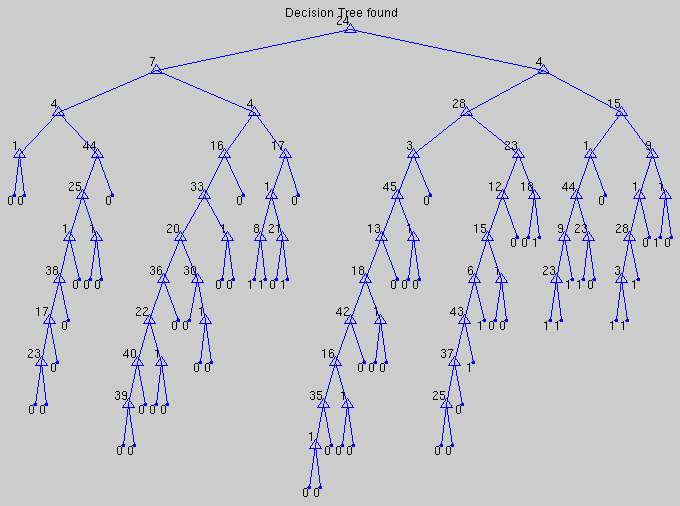
\includegraphics[scale=0.28]{report-images/tree1.png} \\
  Tree for anger \\
  \vspace{\baselineskip}
  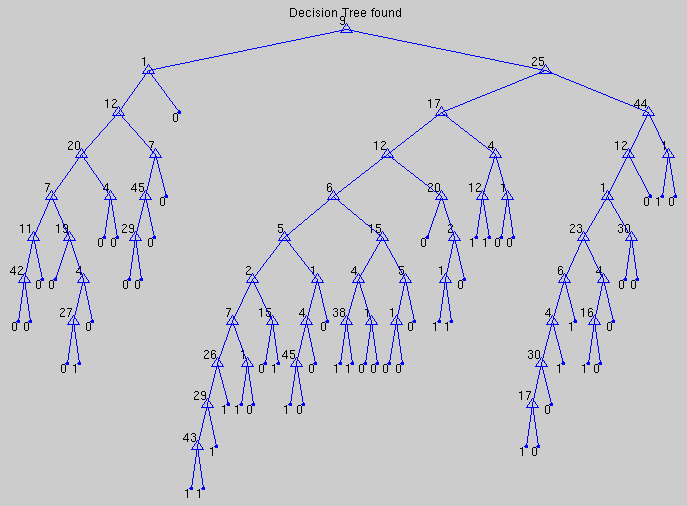
\includegraphics[scale=0.28]{report-images/tree2.png} \\
  Tree for disgust \\
  \vspace{\baselineskip}
  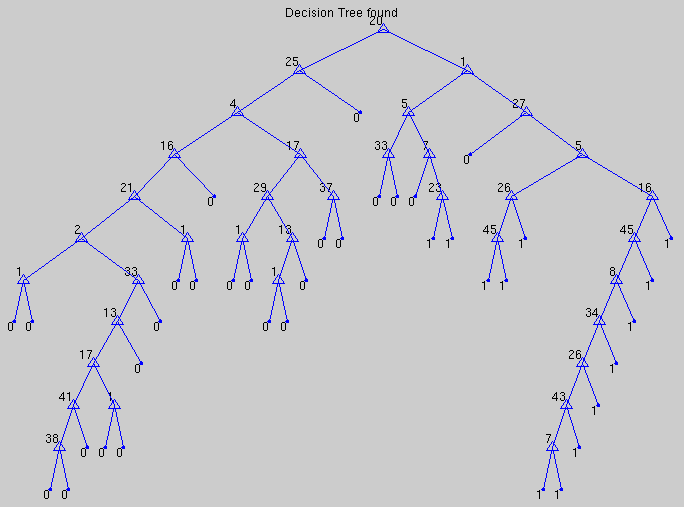
\includegraphics[scale=0.28]{report-images/tree3.png} \\
  Tree for fear \\
  \vspace{\baselineskip}
  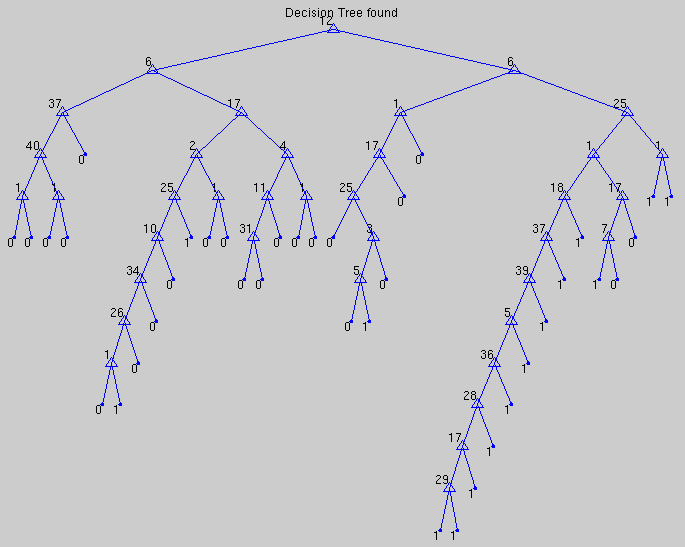
\includegraphics[scale=0.28]{report-images/tree4.png} \\
  Tree for happiness \\
  \vspace{\baselineskip}
  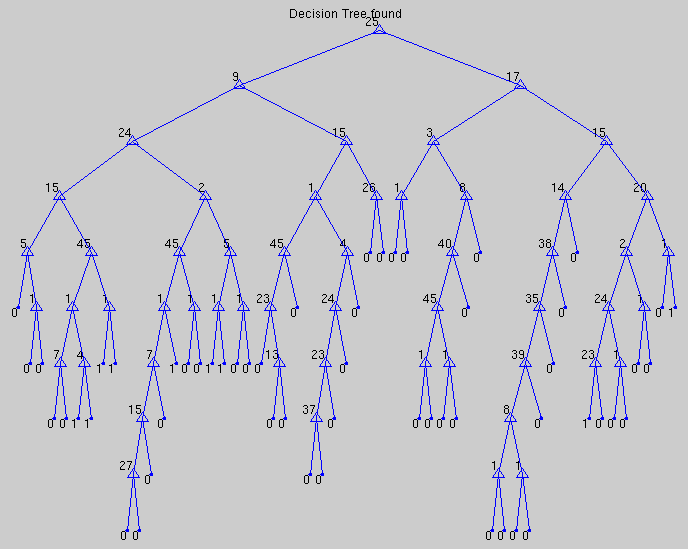
\includegraphics[scale=0.28]{report-images/tree5.png} \\
  Tree for sadness \\
  \vspace{\baselineskip}
  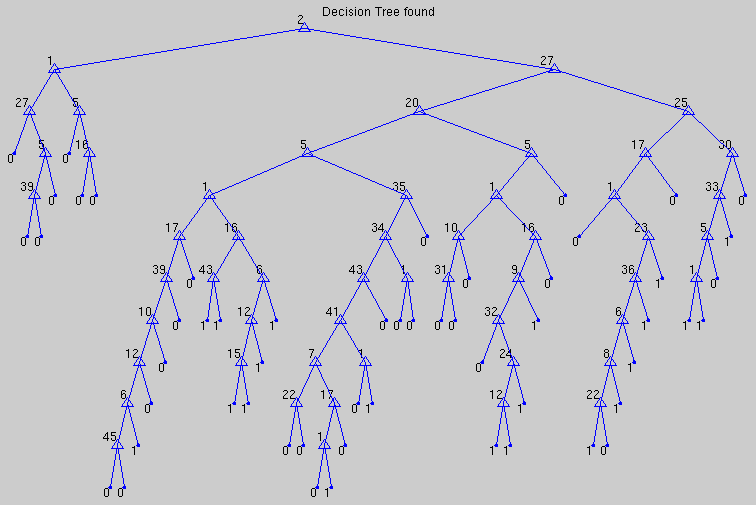
\includegraphics[scale=0.28]{report-images/tree6.png} \\
  Tree for surprise
\end{center}


{\bf Evaluation results} \\
Confusion matrix: The happiness tree was very good, perhaps overfit. Disgust and Happiness were quite often misclassified as well as correctly. They probably produced better trees because there was more data for them. Classification rate: The average classification rate is semi-successful as it succeeds most of the time. But it is far from perfect. Precision/Recall rate:  F-measure: The F measures suggest as suspected that the Disgust and Happiness have well trained trees. Perhaps Sadness and Surprise did not have enough data. Anger is likely an easy emotion to classify given the trees high performance given a relatively small amount of data \\ \\

Confusion matrix: The happiness tree was very good, perhaps overfit. Disgust and Happiness were quite often misclassified as well as correctly. They probably produced better trees because there was more data for them. Classification rate: The average classification rate is semi-successful as it succeeds most of the time. But it is far from perfect. Precision/Recall rate:  F-measure: The F measures suggest as suspected that the Disgust and Happiness have well trained trees. Perhaps Sadness and Surprise did not have enough data. Anger is likely an easy emotion to classify given the trees high performance given a relatively small amount of data \\ \\

\begin{table}
\centering
\begin{tabular}{r r | r r r r r r}
\multicolumn{8}{c}{Predicted class} \\
&  & Anger & Disgust & Fear & Happiness & Sadness & Surprise \\
\hline
& Anger & 7.4 & 1.4  & 0.4 & 2.0  & 0.9 & 1.1 \\
 & Disgust & 1.2 & 15.0 & 0   & 2.1  & 0.6 & 0.9 \\
Actual class & Fear & 0.5 & 2.3  & 3.9 & 1.8  & 0.8 & 2.6 \\
 & Happiness & 0.2 & 2.0  & 0   & 18.8 & 0.1 & 0.5 \\
& Sadness & 0.7 & 2.8  & 0.4 & 2.6  & 4.5 & 2.2 \\
& Surprise & 0   & 4.3  & 1.1 & 6.2  & 0.4 & 8.7 \\
\end{tabular}
\caption{Confusion matrix}
\end{table}

\begin{table}
\centering
\begin{tabular}{l | r r}
Emotion & Recall rate (\%) & Precision rate (\%) \\
\hline
Anger & 56.0606 & 74.0000 \\
Disgust & 75.7576 & 53.9568 \\
Fear & 32.7731 & 67.2414 \\
Happiness & 87.0370 & 56.1194 \\
Sadness & 34.0909 & 61.6438 \\
Surprise & 42.0290 & 54.3750 \\
\end{tabular}
\caption{Recall and precision rates}
\end{table}

\begin{table}
\centering
\begin{tabular}{l | r}
Emotion & \( F_1 \) measure \\
\hline
Anger & 63.7931 \\
Disgust & 63.0252 \\
Fear & 44.0678 \\
Happiness & 68.2396 \\
Sadness & 43.9024 \\
Surprise & 47.4114 \\
\end{tabular}
\caption{F1 measures}
\end{table}

Average classification rate = 0.5808 \\ 


{\bf Ambiguity} \\
There are 2 cases when there needs to be a decision made about classification which cannot be made by the trees themselves. Firstly, it is where none of the trees have returned a positive value, secondly it is when multiple trees positively classify the same example. Initially we chose to randomise the classification, this was our benchmark. The obvious drawbacks of choosing randomly are that it is a complete guess, and should intuitively not be used if there is more information available. Generation of pseudo random numbers is also a rather expensive task if time is a factor. \\

Then we decided to select the value which had been chosen the most so far without contention. This was slightly worse than random on average, it is highly dependent on the order of the data. This method then became superseded by choosing the most common label in the test set. Statistically choosing the most common label should be better on average, but it fared worse when being used for examples that has no classifications. Of course the drawback of this method is that the statistically most common labels need to be known in advance. This method proved to be slightly better than by random on average. \\

Finally, we made a score system for trees when competing against each other. If there were multiple trees all with positive classifications then the tree that was chosen would receive a point if it correctly classified the result, or lose one if it provided a false positive. Then for the next classification the tree with the highest score would be chosen if there was contention. This improved the \( F_1 \) measure, but could not be used when no classes were found. Another drawback is that a different measure must be used the first time there is contention as there are no scores, and this can have a large impact on the path of evaluation. Also, it may not always be possible to get immediate feedback on the classification whilst learning, which would not make this possible. This method is also bound by the complexity of sorting the order of label priorities (n log n), so it may not be the best choice if there is a very large number of labels, and time is a factor. \\

<<<<<<< HEAD
Finally, we made a score system for trees when competing against each other. If there were multiple trees with positive classifications, then the tree that was chosen would receive a point if it correctly classified the result, but lose one if it provided a false positive. For the next classification, the tree with the highest score would be chosen if there was contention. This improved the \( F_1 \) measure, but could not be used when no classes were found. Another drawback is that a different measure must be used the first time there is contention, since there are no scores, and this can have a large impact on the path of evaluation. Also, it may not always be possible to get immediate feedback on the classification whilst learning, which would impose limits on its usefulness. This method is also bound by the complexity of sorting the label priorities (n log n), so it may not be the best choice if there are a very large number of labels, and time is a factor. \\

If we had more time, I would like to have trained a decision tree to choose which label to trust in the event of multiple positives, or even in other cases (for instance, if it was always the case that when the two positive-valued trees were Anger and Surprise, then the actual label was Happy). It is worth noting that this would require a much larger sample of data. \\ \\
=======
If we had more time, I would like to have trained a decision tree to choose which label to trust in the event of multiple positives, or even in other cases (for instance if it was always the case that if the two trees to return positive were Anger and Surprise then the true label was Happy, if all the other trees returned negative). It is worth noting that this would require a much larger sample of data. \\
>>>>>>> 0ce18fc41967fc8d7924d1dc3d83f4b55b9bf47c

{\bf Pruning} \\
The pruning\_examples function shows a graph where tree pruning is used on a decision tree built using the default matlab libraries. We imagine tree pruning will first remove branches that result in the same value no matter the value of the attribute split on.

The pruning algorithm used is resubstitution pruning which substitutes leaf nodes with the most common attribute, until the error value is intolerably high.

The cost variable on the y-axis is the average number of comparisons for each classification. This is calculated by summing the probability that a leaf node is reached, by the cost it took to reach.

We think that this cost is calculated based on trees of different sizes, showing the value of cost for each size of tree. The blue line is probably without using pruning, and the red line is with using pruning.

The optimal tree size when using the pruning algorithm is one where the cost is as small as possible, yet still having an error rate of the tree using cross validation. \\
<<<<<<< HEAD

\begin{center}
  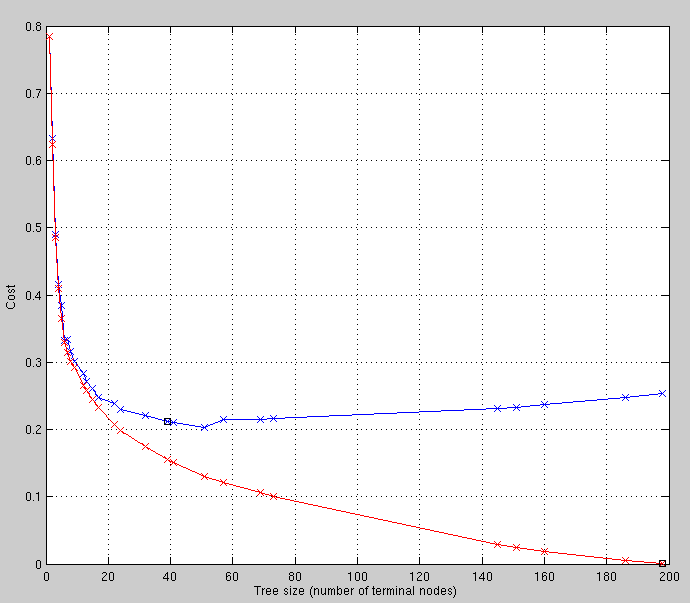
\includegraphics[scale=0.6]{report-images/pruning.png}
\end{center}
=======
>>>>>>> 0ce18fc41967fc8d7924d1dc3d83f4b55b9bf47c


\newpage

{\bf Code Flowchart} \\
\begin{center}
  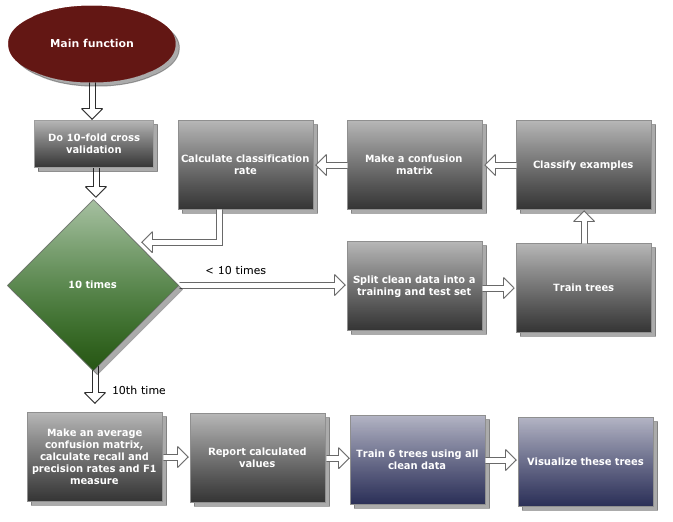
\includegraphics[scale=0.6]{report-images/flowchart.png}
\end{center}

\end{document}
